\chapter{Testing}

Using the environment outlined in \ref{sec:testing_environment}, we can test the framework against the objectives outlined in \ref{ch:objectives}.
This chapter will outline the tests performed and the results of those tests.

\section{Channel selection and adaption}
\label{sec:channel_selection_and_adaption}

Plot traffic of env and covert channel, ALL IP -> ALL TCP, watch switch

\section{Detecting and recovering from failures}
\label{sec:detecting_and_recovering_from_failures}

No idea how to plot this, but it works.

\section{Recovering from a communication channel failure}
\label{sec:recovering_from_a_communication_channel_failure}

Show that the framework can recover from a channel failure, don't know how.

\section{Testing the covertness of communication}

Bit distribution, record payloads (and MP) and compare to a uniform distribution.

\section{Detecting the channel with knowledge of its implementation}

Script that identifies the channel, evaluate false positives, also evaluate the retrospective identification vs real-time identification.

\section{Transmission padding}
\label{sec:padding_testing}

The types of padding, outlined in \ref{sec:transmission_padding}, are tested in this section.

The padding that works with a 1 followed by 0's for the remaining space will be referred to as "short" padding, and the padding proposed will be referred to as "covert" padding.

The drawback of covert padding over short padding is the additional space required to transmit the padding, however, due to the block size of AES encryption, the number of additional packets sent by this padding is negligible:

\begin{figure}[h]
    \centering
    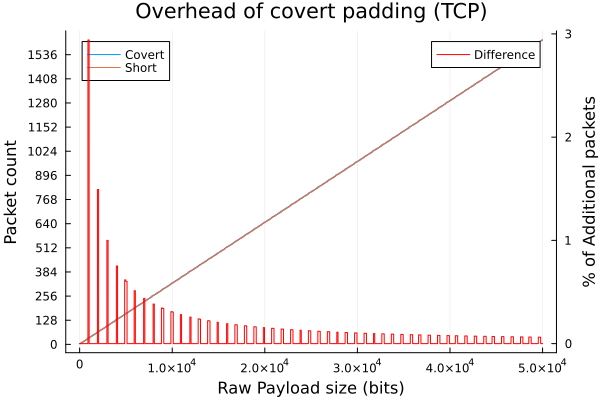
\includegraphics[width=0.7\textwidth]{fig/padding_size_TCP.png}
    \caption{The size of the padding required for a given payload size (TCP)}
    \label{fig:padding_size_TCP}
\end{figure}

\begin{figure}[h]
    \centering
    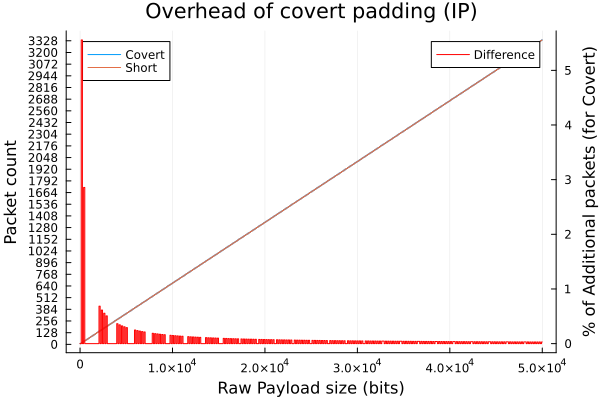
\includegraphics[width=0.7\textwidth]{fig/padding_size_IP.png}
    \caption{The size of the padding required for a given payload size (IP)}
    \label{fig:padding_size_IP}
\end{figure}

We can see here that the use of covert padding has very little effect on the number of packets sent, with the maximum being 5\% more packets sent for a payload (for IP). It is evident that the covert padding method is more effective for TCP, but for both protocols, they do not outperform the short padding method. By taking the number of payloads that require an extra packet to be sent, and dividing it by the total number of payloads, we get the percentage of packets that require an extra packet to be sent, multiplying that by the average percentage increase in packets sent, we can find the approximate overhead of the covert padding method:

Where $n$ is the number of payloads, $d$ is the number of $p$ that require an extra packet to be sent, $p_s$ is the average percentage increase in packets sent, and $o$ is the average overhead of the covert padding method, expressed as a percentage.

\begin{equation*}
    o = \frac{d}{n} * p_s * 100
\end{equation*}

The overhead for packets for TCP and IP is 1.02\% and 2.71\% respectively.

Where the covert padding method performs is in the distribution of the bits, where fields are supposed to be random, or unique, the percentage of 0's should be approximately 50\%, however, with short padding, this is not the case:

\begin{figure}[h]
    \centering
    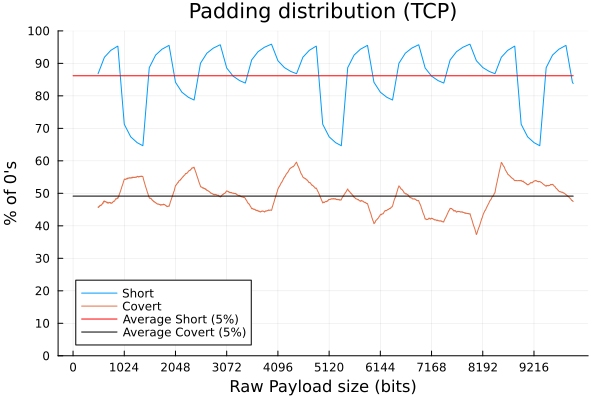
\includegraphics[width=0.7\textwidth]{fig/padding_distribution_TCP.png}
    \caption{A comparison of bit distributions in the TCP header with short padding and covert padding}
    \label{fig:padding_distribution_TCP}
\end{figure}

\begin{figure}[h]
    \centering
    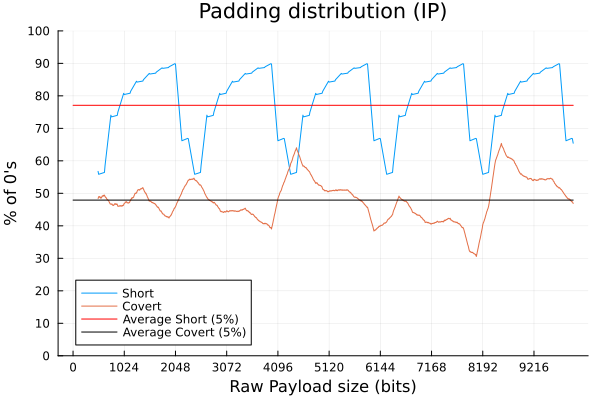
\includegraphics[width=0.7\textwidth]{fig/padding_distribution_IP.png}
    \caption{A comparison of bit distributions in the IP header with short padding and covert padding}
    \label{fig:padding_distribution_IP}
\end{figure}

We can see here that the covert padding method is much closer to the ideal distribution than the short padding method. We can also see that again, the larger field of the TCP header is better suited to the covert padding method, with a tighter distribution than the IP header. The covert headers are not perfect, because the size of the data always starts with a 0, which is required for the padding to be removed, however, this difference is negligible and would not be statistically significant.

